\section{Projection Insertion}
\label{sec:field-reduction}

% Intro/Motivation 
A common optimization in data processing is to early remove intermediate values that not needed in later phases of the computation. It has been implemented for SQL databases for a long time, and has recently been added to the Pig framework. This optimization requires all field accesses in the program to be explicit. A library can provide this, but the programmer needs to specify it explicitly - which is error prone and tedious. 

% It used to be a tip to do this optimization manually for Pig before they added this optimization, the tip still is valid for cascading and scalding.

% description of supported types
In \tool we support this optimization for algebraic data types, more specifically final immutable Scala classes with a finite level of nesting. Our approach does not require special syntax or access operators and supports method declarations on a data type like  regular Scala classes. While implementing our benchmarks we found this to be a reasonably expressive model for big data programming. The DSL user needs to supply class declarations, from which we generate all the necessary code for its use in \tool. The generated code includes a parsing method, to which the user has to supply a regular expression in case the data is stored in text form. Our IR describes all field accesses explicitly and we can generate highly specialized code for these types including serialization schemes and other glue code for the back-ends we support.

% explaining the lingo and high level overview of the algorithm.
In section \ref{sbusec:lms-optimizations} we have shown how LMS optimizes these classes within the same program scope. In \tool we endorse a declarative programming model with many short functions - which each have their own scope - as these are easier to read and optimize. Each operation has an input type and an output type, and may have a function - or more correctly a closure. Operations are chained together to form a data flow graph without cycles, so each operation has either successors or predecessors. We define paths to be the chain of field dereferences needed to access a certain value within a a scope's input type. A field access describes such a path as a list of strings. See \ref{fig:type_tree} for a small example. \\
For our projection insertion algorithm we therefore need to analyze all scopes to get a list of all field accesses for it. The algorithm goes backwards through the data flow graph and computes for each operation the field reads to propagate them to its predecessors. For correct handling of loops we apply this until we reach a fixpoint. We use this analysis to insert projections before an operation that serializes each object or stores it in memory.
\begin{figure*}
\begin{subfigure}[b]{.5\linewidth}
\begin{lstlisting}[name=code, caption=Types for field access example]
case class A(id: String, b: B)
case class B(id: String)  
val t = ("tuple", A("a", B("b"))) 
t: scala.Tuple2[String, A]
\end{lstlisting}
\centering
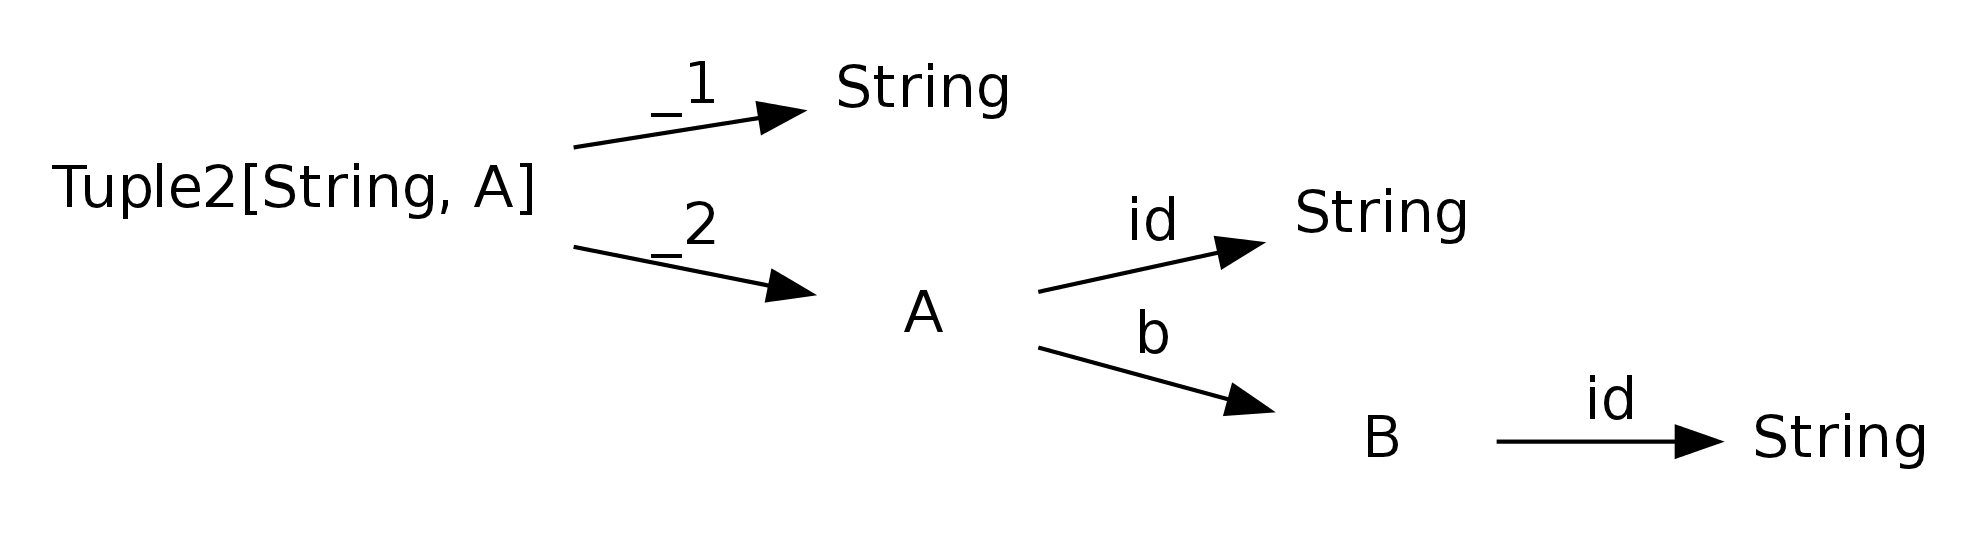
\includegraphics[width=\linewidth]{dot/access.png}
\caption{Visualization of the type. The nodes are the types at each level, the edges describe a field dereference. The leafs are always primitive types, and the path is formed by concatenating the edge labels. At the leafs, the value in the above example is given. An example path description is ``\_2.b.id''}
\end{subfigure}
\label{fig:type_tree}
\end{figure*}
\\
% explaining the analysis
For the analysis of one operation, we used these primitives which can be combined:
\begin{itemize}
\item Create field accesses for all fields nested within a type. For example a \code{DList.save(....)} on A would generate reads for id and b.id. 
\item Rewrite accesses from predecessors according to semantics of the operation. For example, the filter operation will never change the object itself, so all field accesses from a filters successors must be propagated to its predecessors. A GroupByKey operation on the other hand always reads all parts of the key, and additionally changes all field accesses of the form \code{.\_2.iterable.x to .\_2.x}, as the iterable is introduced by the operation itself and is known to conserve the instances.
\item Analyze a closure scope. A closure can be analyzed by filtering all the expressions contained in its scope and checking if they (recursively) read fields from the input of that scope. As such we do not actually analyze all code, analyzing the field reads is enough. 
\item Replace the output symbol of a scope with a synthesized one which only contains the later needed fields. See example \todo{sample} for a simple illustration. We need this primitive for the analysis of closures which can do arbitrary transformation, but can reuse it as well for the later projection insertion itself. For a map closure we replace the output, and then analyze the field reads, otherwise some field reads would be in the scope to fill in values into the output which are no longer needed afterwards. This new closure, after dead code elimination, can then be analyzed by the closure analysis primitive.
\end{itemize}
Table \ref{table:field_reduction} shows how these primitives are combined to form the rules of the most important operations on Dlist.

\todo{Each clause needs to be either well known in the scientific discourse - cited if significant, or mentioned earlier in the paper}

\todo{From here on not yet revised}
\bigskip

It should be noted that the soundness of our algorithm depends on the optimizations in LMS itself. LMS inlines functions
by default, provides dead code elimination and a field read from a constructor invocation will be reading the
expression directly, thus rendering the intermediate object creation dead. Additionally we rely on dead code
elimination. 

An advantage of our scheme is that it does not require a full code analysis.\todo{why}

\todo{}

\begin{table}
    \begin{tabular}{l|l|l}
    
        ~            & Field Reads                                                                           & barrier \\ \hline
        filter       & All of successor + closure reads                                                      & ~       \\ 
        flatmap      & All of the closure with a replaced output                                             & ~       \\ 
        map          & All of the closure with a replaced output                                             & ~       \\ 
        join         & Adds accesses to the key, distributes accesses to values to correct predecessor       & x       \\ 
        group by key & Adds access to the key, rewrites accesses to the value's iterable to the value itself & x       \\ 
        reduce       & All accesses from the closure are translated to access of the value's iterable        & ~       \\ 
        save         & Generate accesses for all field reads                                                 & ~       \\ 
        sort         & TODO                                                                                  & TODO    \\ 


    \end{tabular}
    \label{table:field_reduction}
\end{table}

